\section{Heimautomatisierungsserver}

\begin{frame}{Heimautomatisierungsserver}{Systemaufbau}
	\begin{figure}
	\centering
	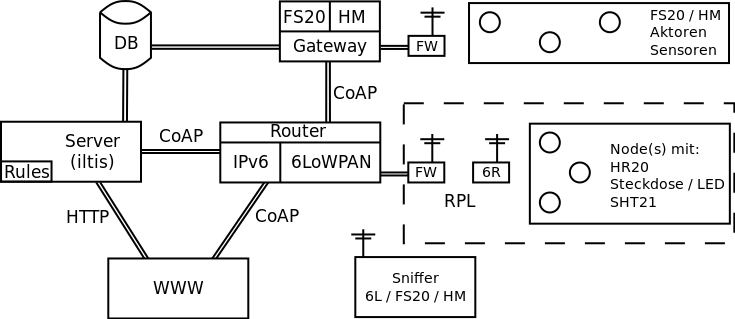
\includegraphics[width=\linewidth]{Systemaufbau}
	%\linebreak
	%\emph{}
	\end{figure}
\end{frame}

\begin{frame}{Heimautomatisierungsserver}{Steuerungsserver und Gateway-Server}
	\begin{block}{Steuerungsserver}
		\begin{itemize}
		\item 	Pairing neuer Geräte
		\item 	Pflegen der angemeldeten Geräte und dessen Sensoren/Aktoren
				(in einer Datenbank)
		\item 	Regelkreis bestimmt Automatisierungsprozess (Regelwerk)
		\end{itemize}
	\end{block}
	\begin{block}{Gateway-Server}
		\begin{itemize}
		\item 	Schnittstelle zwischen CoAP und proprietären Sensornetzen
				\eg(FS20, HomeMatic)
		\item 	Nutzen der Datenbank zur Kategorisierung
		\item 	Caching von Sensorwerten
		\end{itemize}
	\end{block}
\end{frame}

%\subsection{Regelwerk}

%\begin{frame}{Heimautomatisierungsserver}{Regelwerk}
%	\begin{block}{Automatisierung per Regelwerk}
%		\begin{itemize}
%		\item 	\todo{Stand der Technik, vorhandene Lösungen!}
%		\end{itemize}
%	\end{block}

%	\begin{block}{XML als Datenformat}
%		\begin{itemize}
%		\item 	weit verbreitetes Datenformat
%		\item 	Parser in vielen Programmiersprachen vorhanden
%		\item 	XML Schema Validation
%		\item 	in Blockdarstellungen überführbar (für Nutzer)
%		\end{itemize}
%	\end{block}
%\end{frame}

\begin{frame}{Heimautomatisierungsserver}{Anfrage an das Sensornetz}
	\begin{block}{direkte CoAP-Anfragen}
		\begin{itemize}
		\item 	in das 6LoWPAN-Netz ohne Probleme
		\item 	in das FS20/HomeMatic-Netz über Gateway
		\end{itemize}
	\end{block}
	\begin{block}{HTTP-Anfragen auf dem Server}
		\begin{itemize}
		\item 	Mapping von HTTP auf CoAP
		\end{itemize}
	\end{block}
	\begin{block}{Webserver}
		\begin{itemize}
		\item 	Statistiken
		\item 	Erstellung von Regeln
		\item 	Übersicht über alle Sensoren und Aktoren
		\end{itemize}
	\end{block}
\end{frame}

